\appendix

\chapter{图表}

\begin{figure}[ht]
  \vspace{-1.5cm}
  \centering
  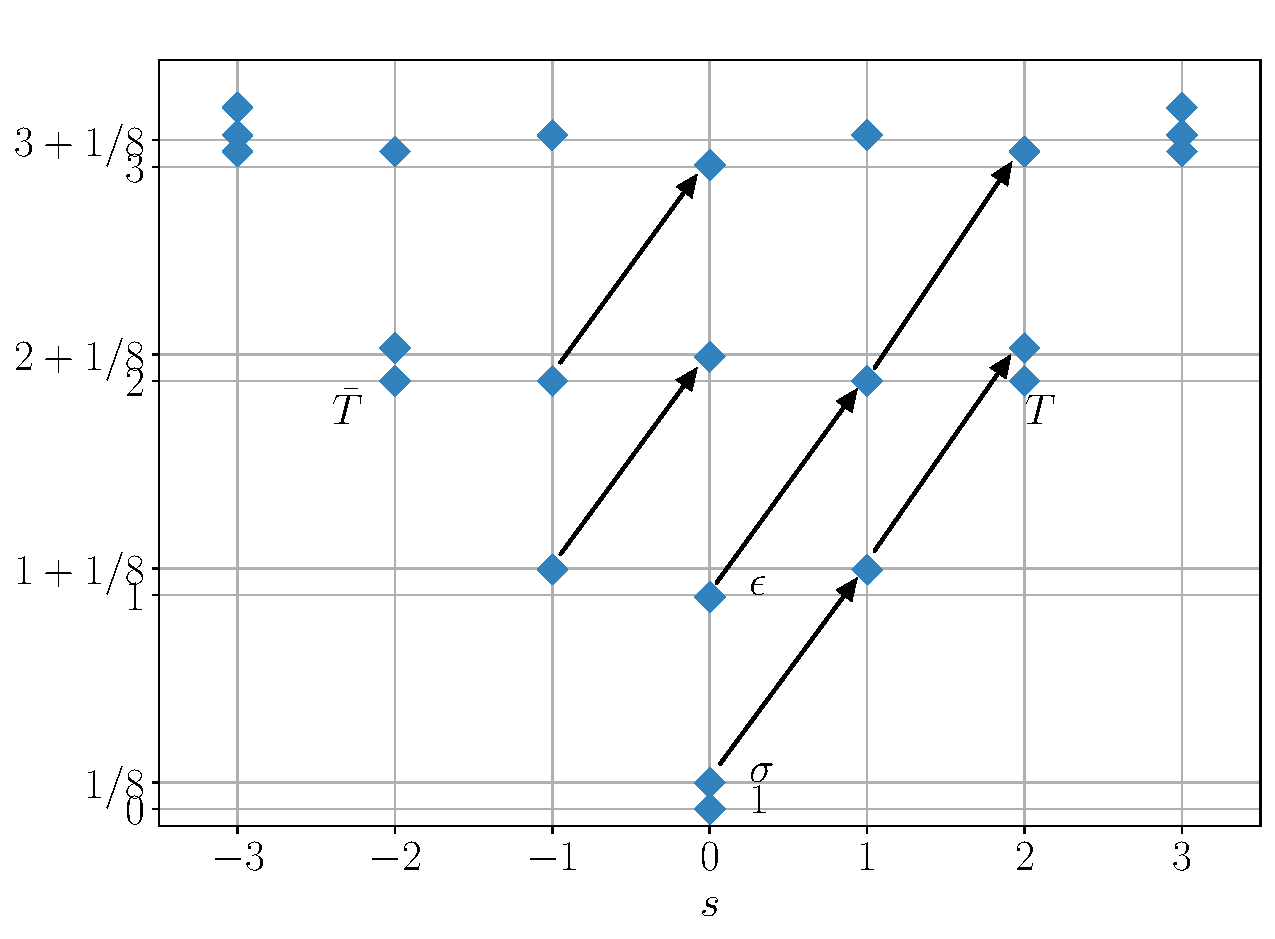
\includegraphics[width=0.45\textwidth]{images/virasoro/ising-lm1.pdf}    \quad
  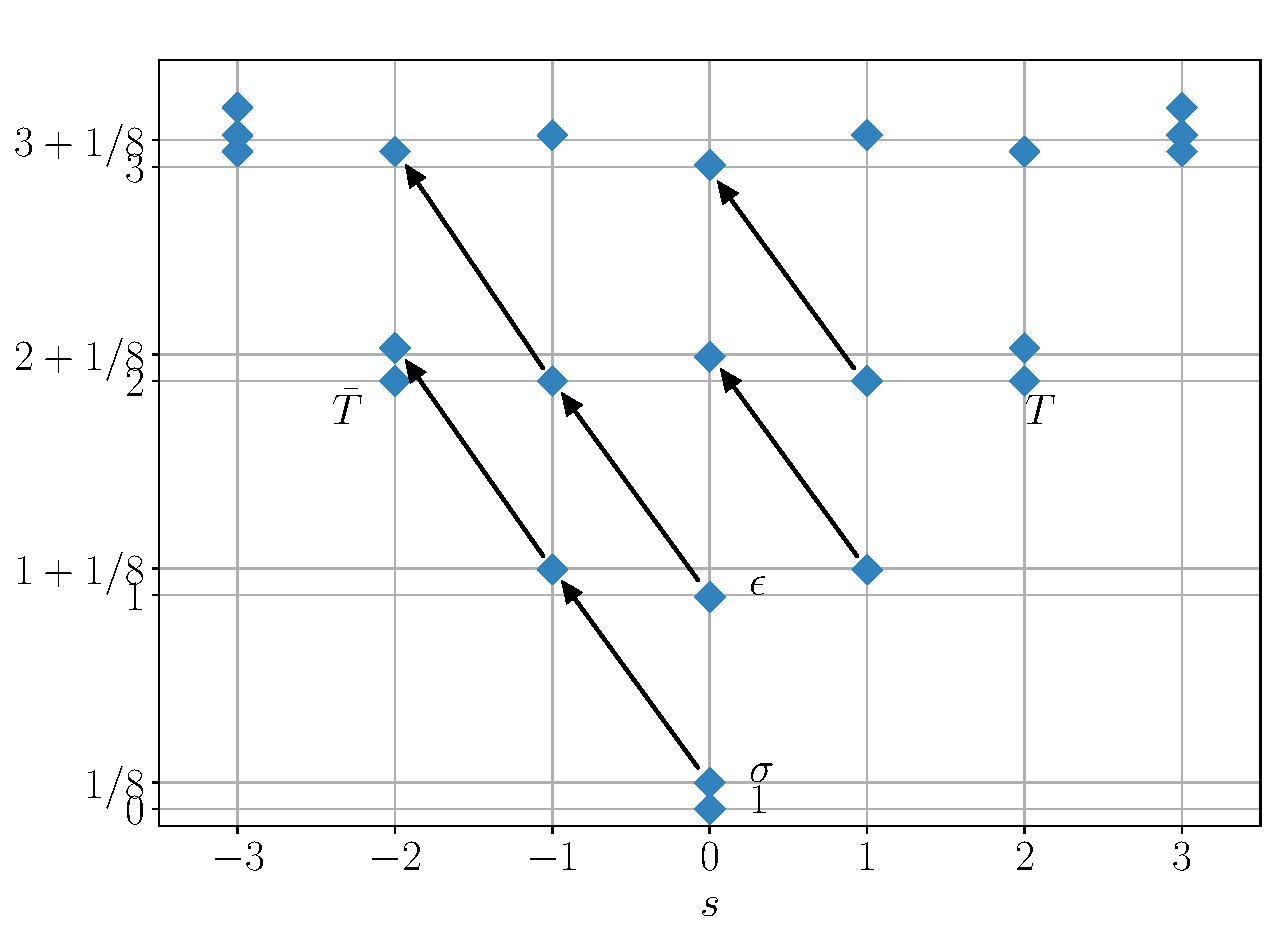
\includegraphics[width=0.45\textwidth]{images/virasoro/ising-lbarm1.pdf} \\
  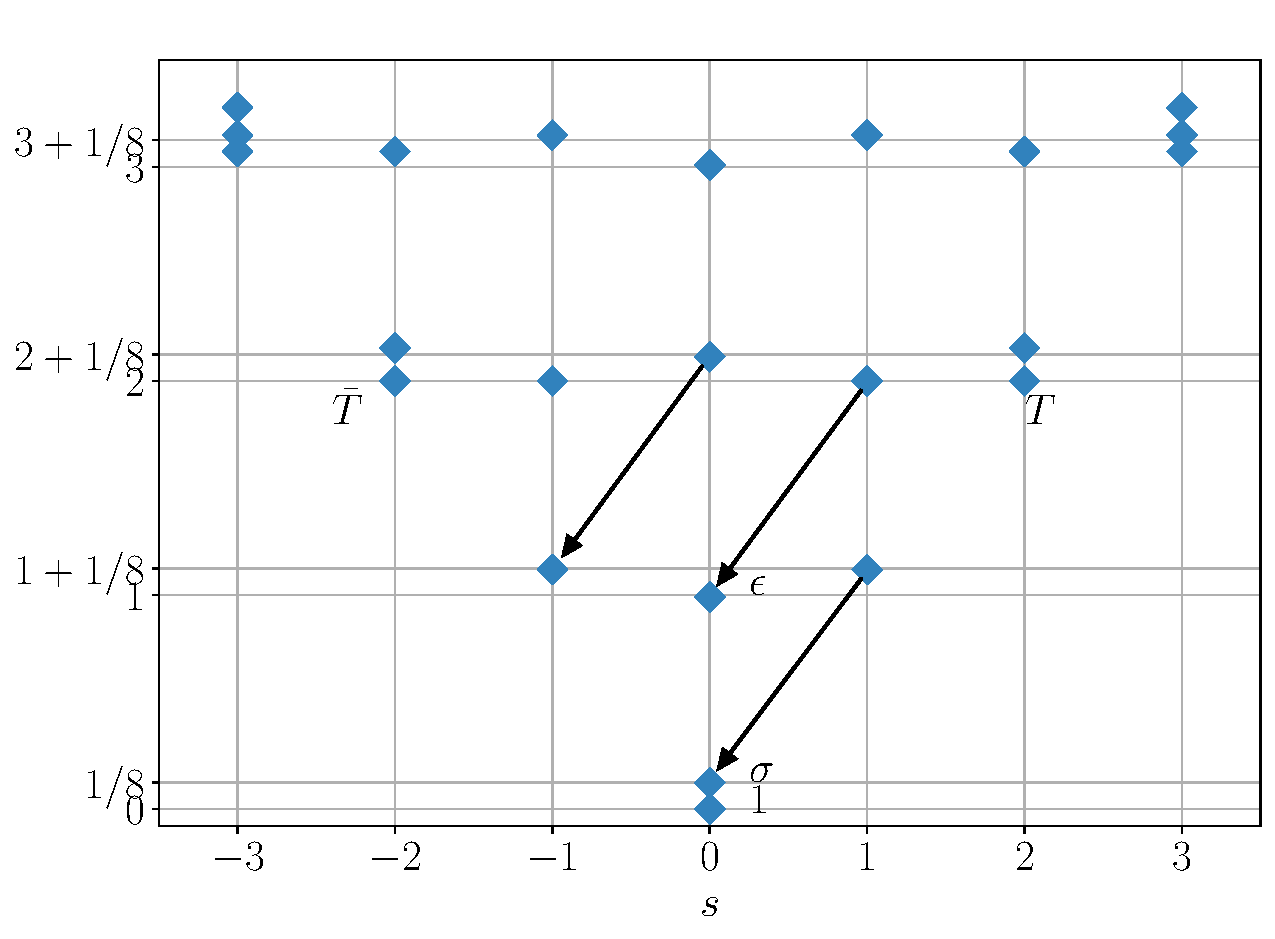
\includegraphics[width=0.45\textwidth]{images/virasoro/ising-l1.pdf}     \quad
  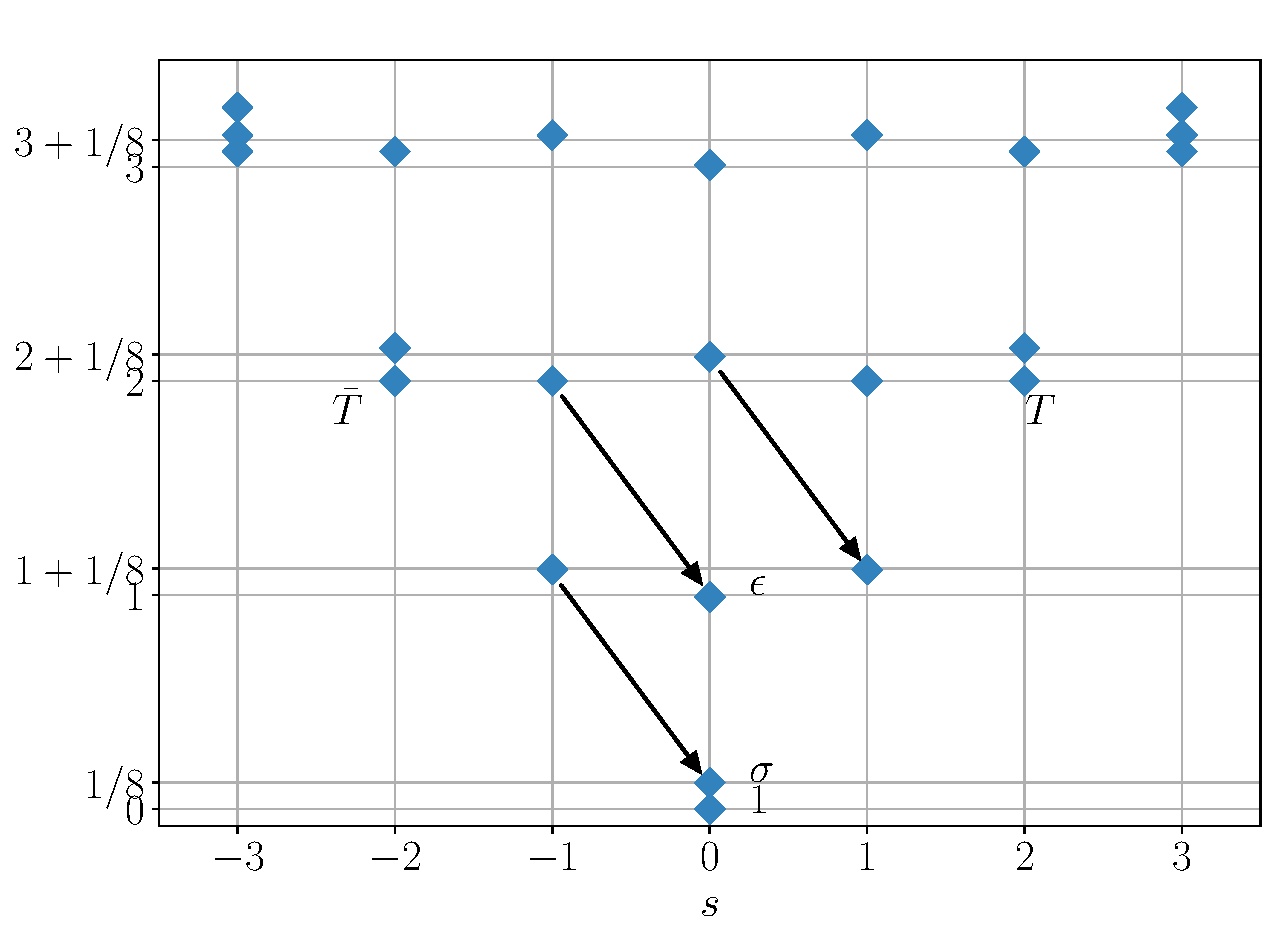
\includegraphics[width=0.45\textwidth]{images/virasoro/ising-lbar1.pdf}  \\
  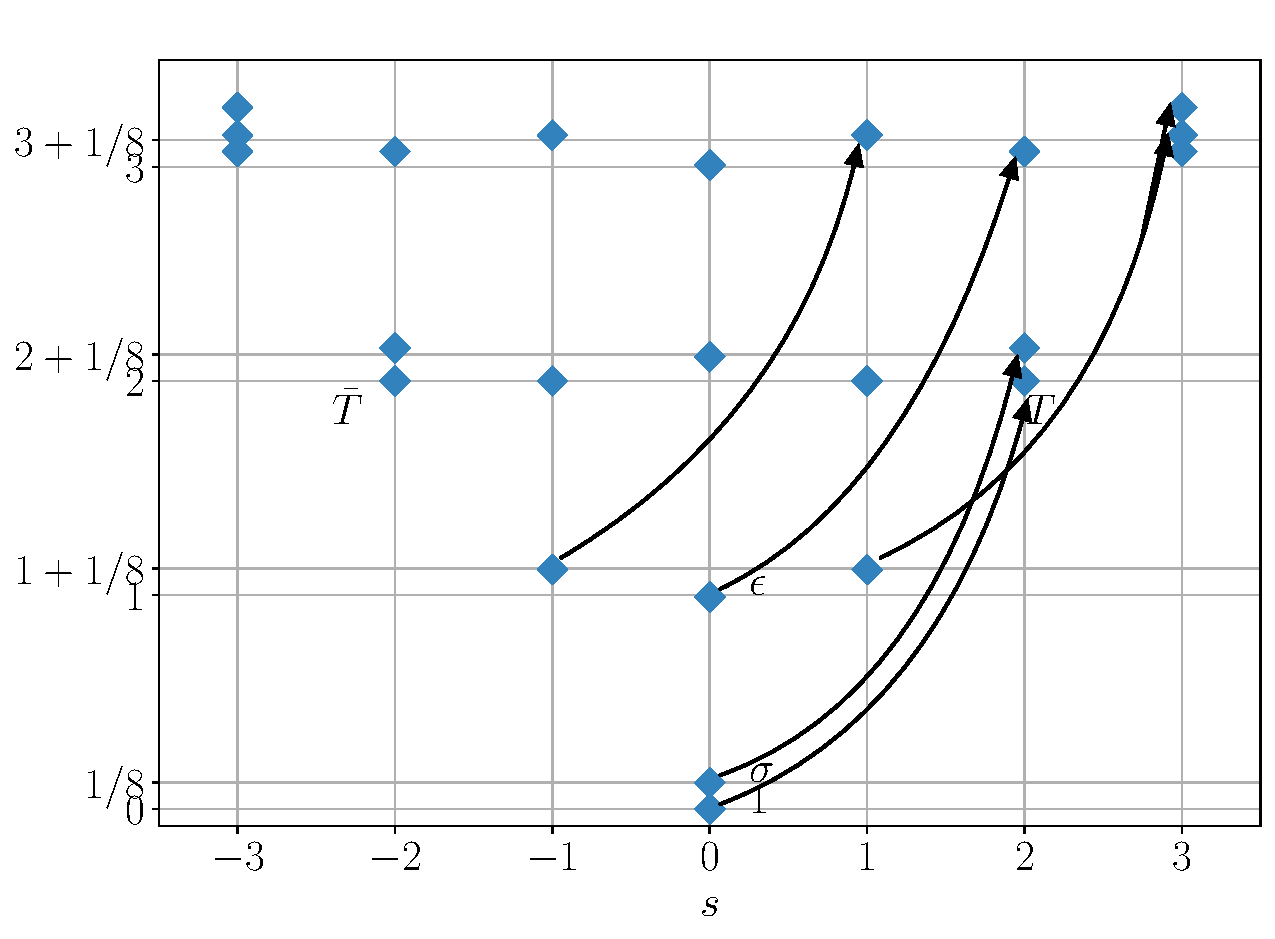
\includegraphics[width=0.45\textwidth]{images/virasoro/ising-lm2.pdf}    \quad
  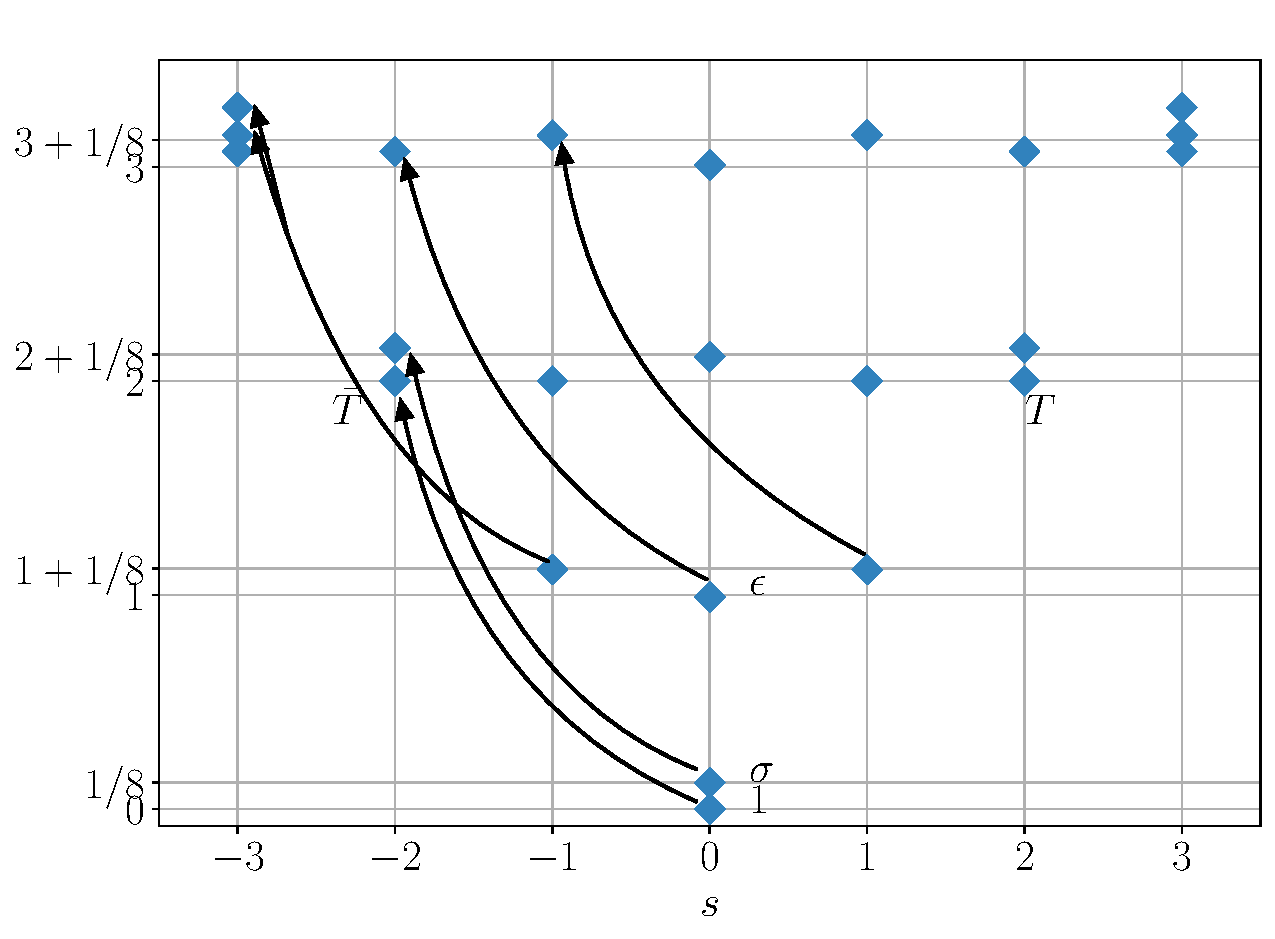
\includegraphics[width=0.45\textwidth]{images/virasoro/ising-lbarm2.pdf} \\
  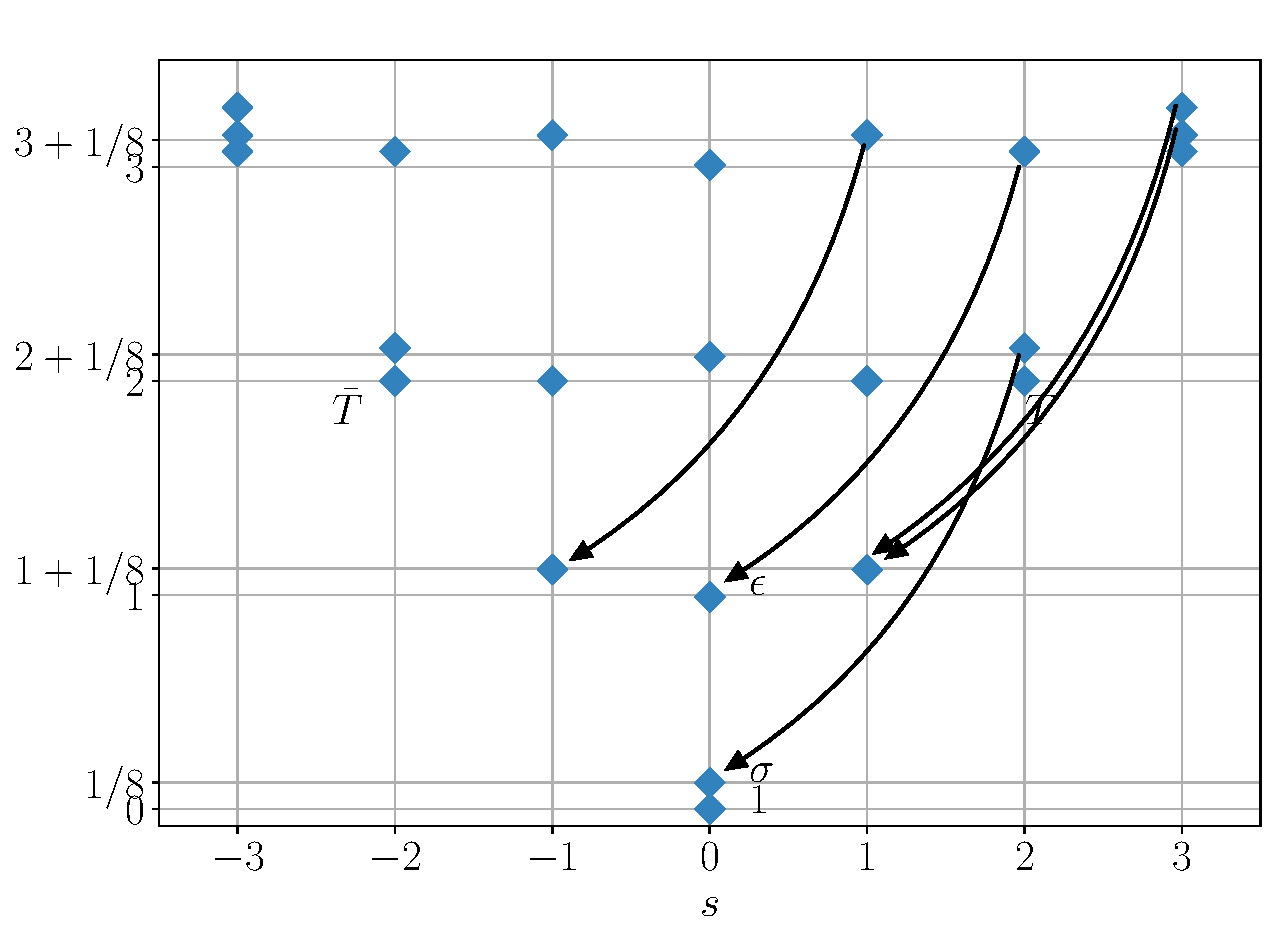
\includegraphics[width=0.45\textwidth]{images/virasoro/ising-l2.pdf}     \quad
  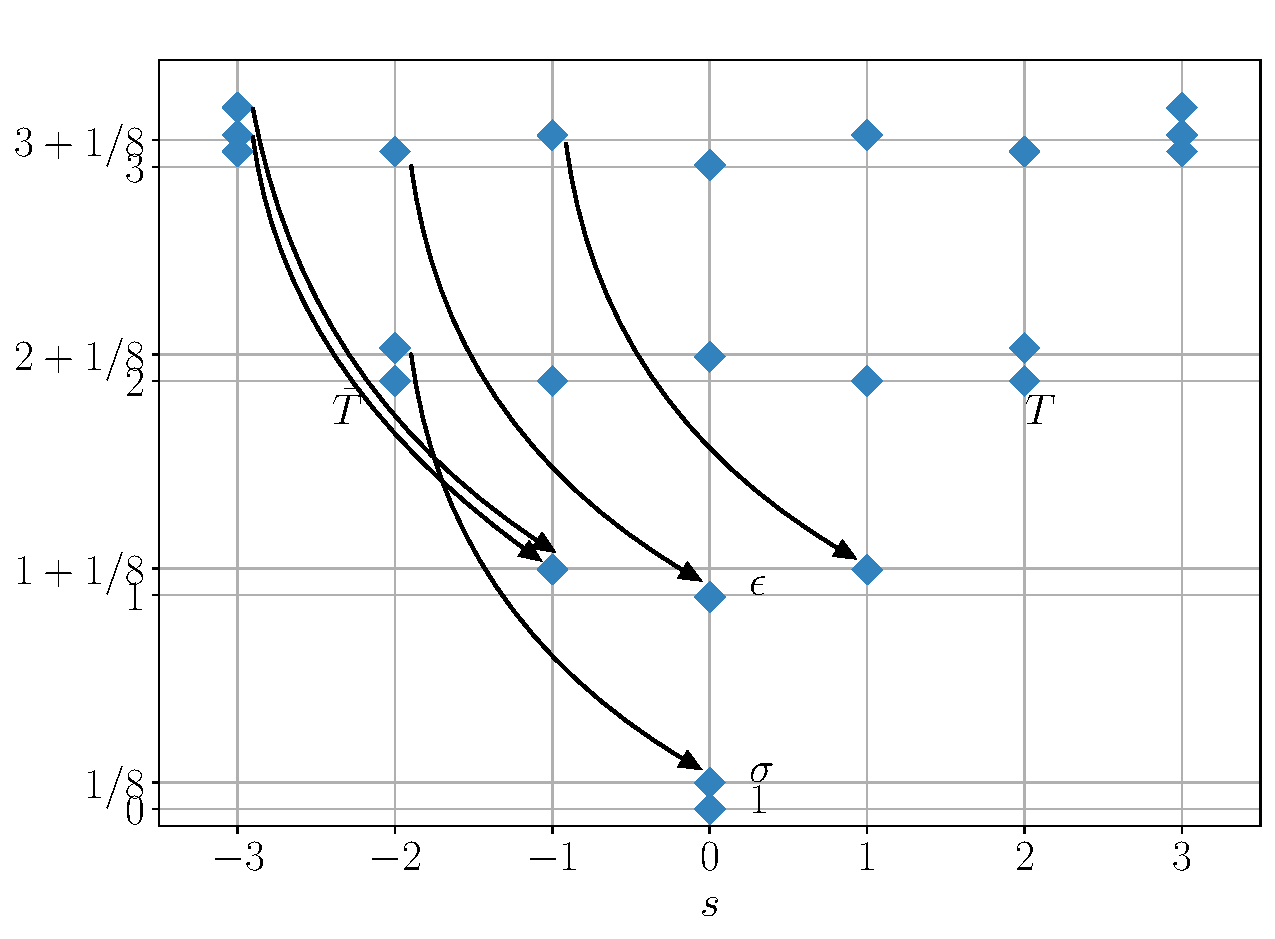
\includegraphics[width=0.45\textwidth]{images/virasoro/ising-lbar2.pdf}
  \caption[Virasoro 算符在 Ising 模型能谱上的作用示意图]{Virasoro 算符在 Ising 模型能谱上的作用示意图。图片来源:\parencite{wang2022virasoro}。}
  \label{fig:ising-virasoro-all}
\end{figure}

\begin{figure}[ht]
  \centering
  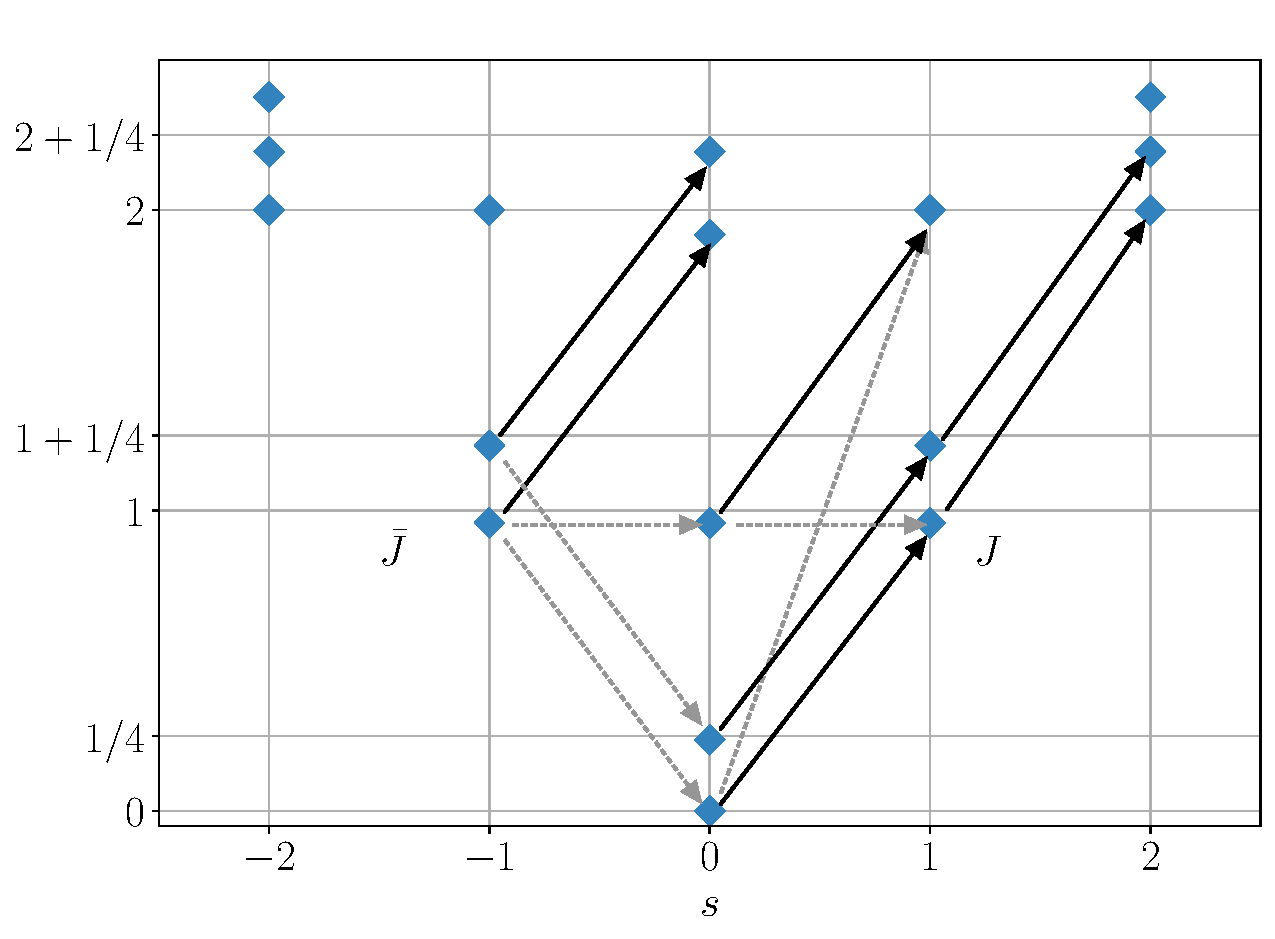
\includegraphics[width=0.45\textwidth]{images/virasoro/dimer-jm1.pdf}    \quad
  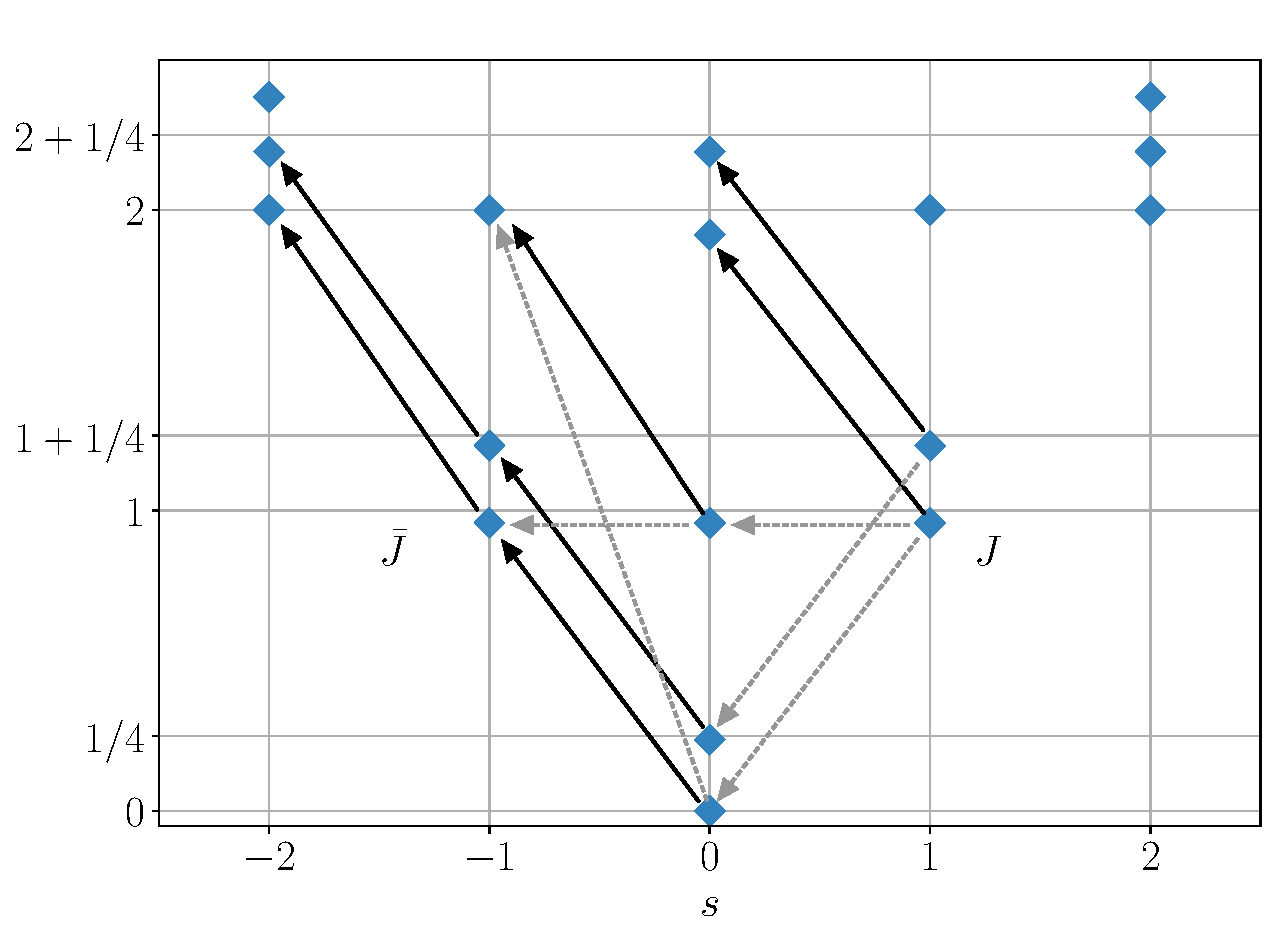
\includegraphics[width=0.45\textwidth]{images/virasoro/dimer-jbarm1.pdf} \\
  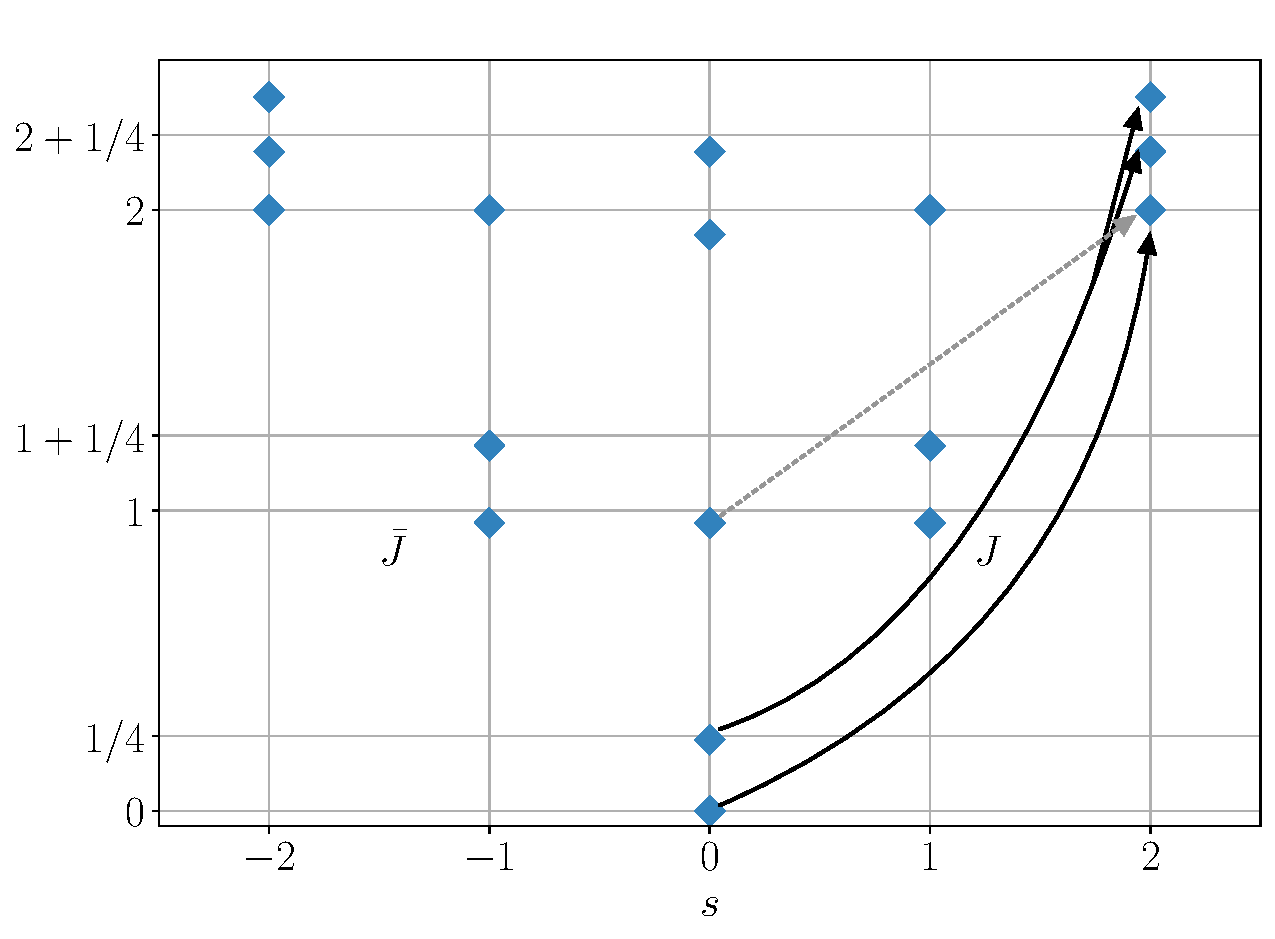
\includegraphics[width=0.45\textwidth]{images/virasoro/dimer-jm2.pdf}    \quad
  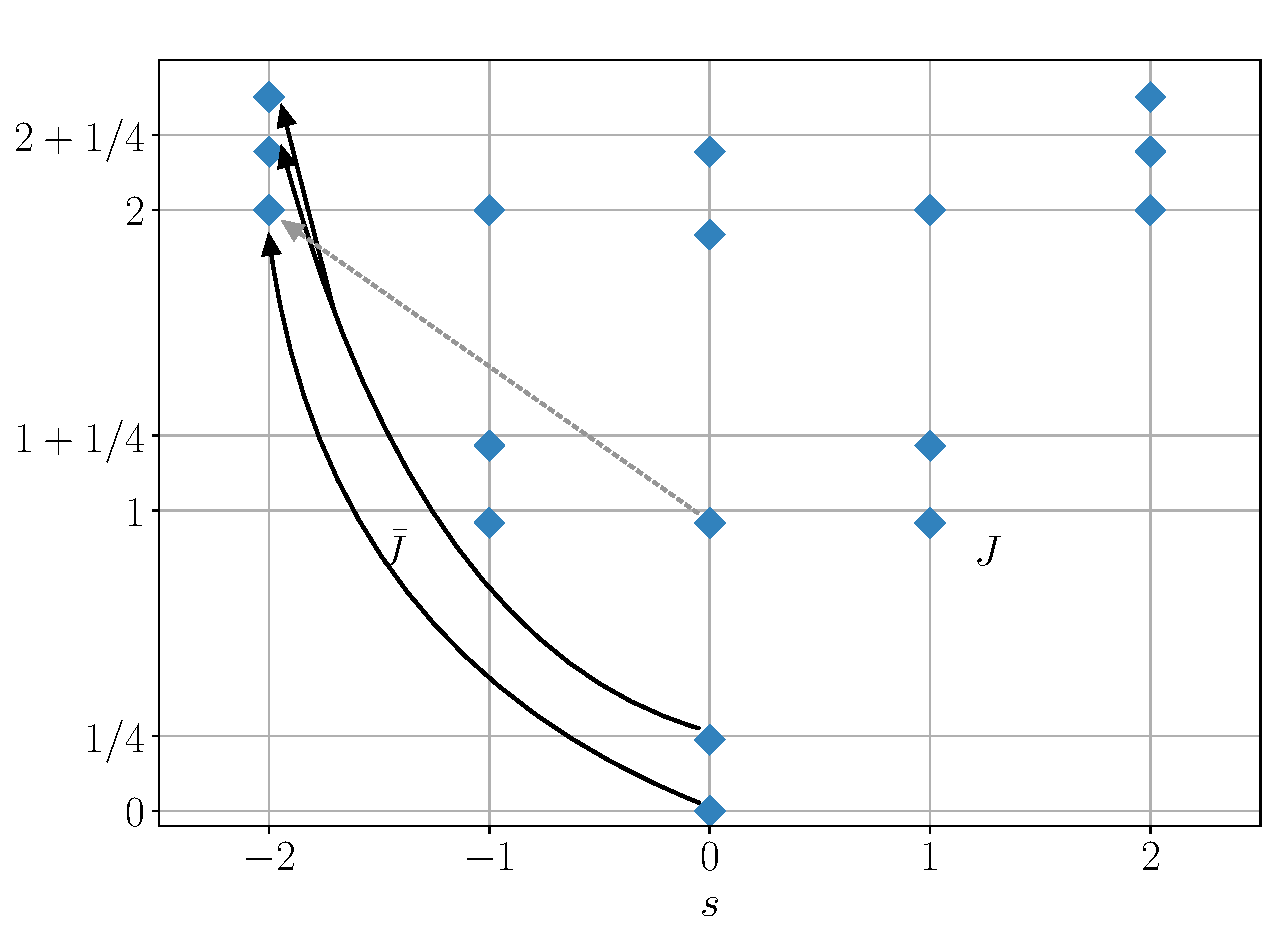
\includegraphics[width=0.45\textwidth]{images/virasoro/dimer-jbarm2.pdf}
  \caption[Kac--Moody 算符在 dimer 模型能谱上的作用示意图]{Kac--Moody 算符在 dimer 模型能谱上的作用示意图。图片来源:\parencite{wang2022virasoro}。}
  \label{fig:dimer-kac-moody-all}
\end{figure}

\begin{figure}[ht]
  \centering
  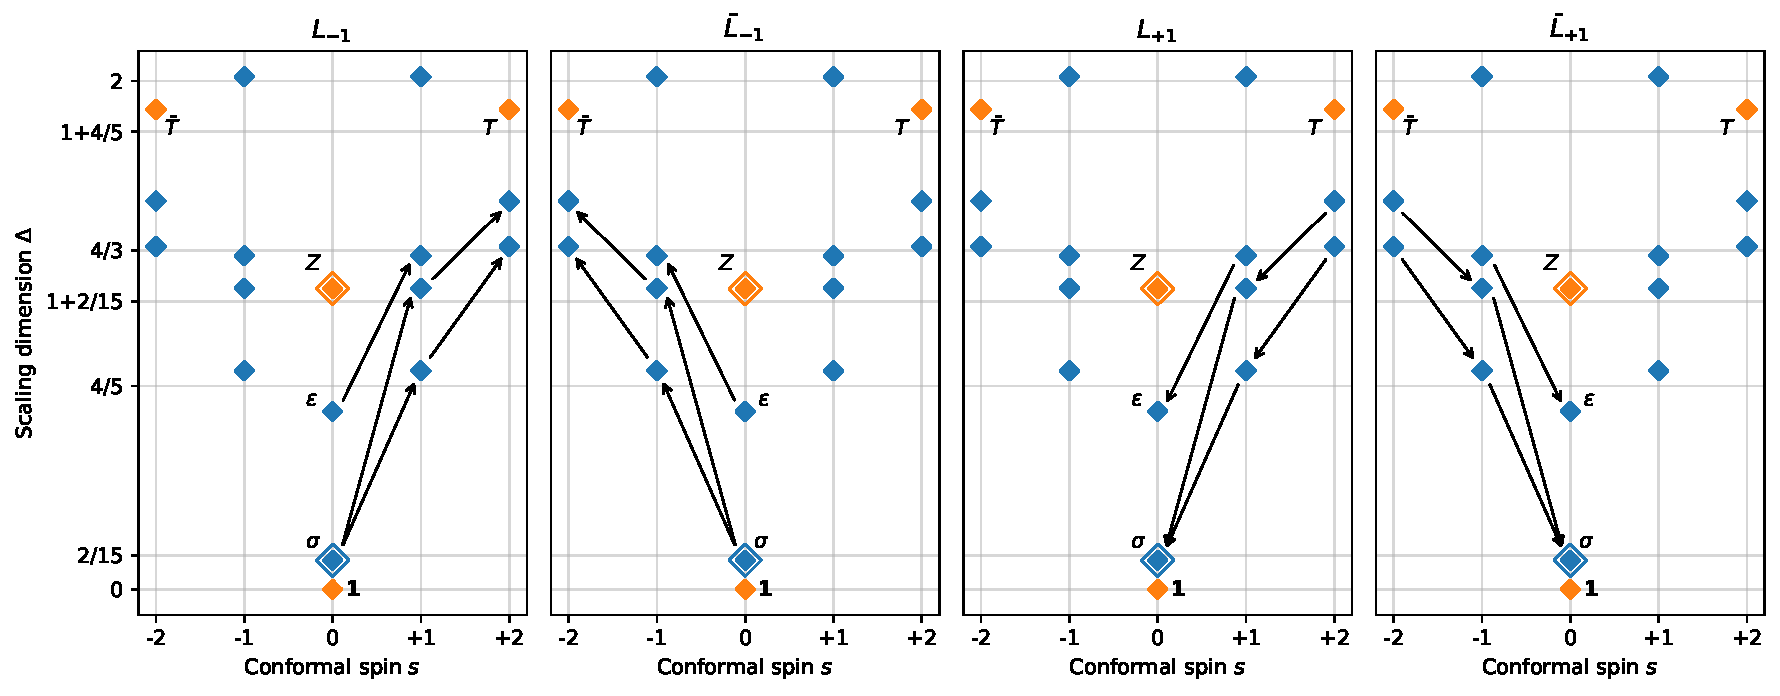
\includegraphics[width=\textwidth]{images/fibonacci/fib-virasoro-all-1.pdf} \\
  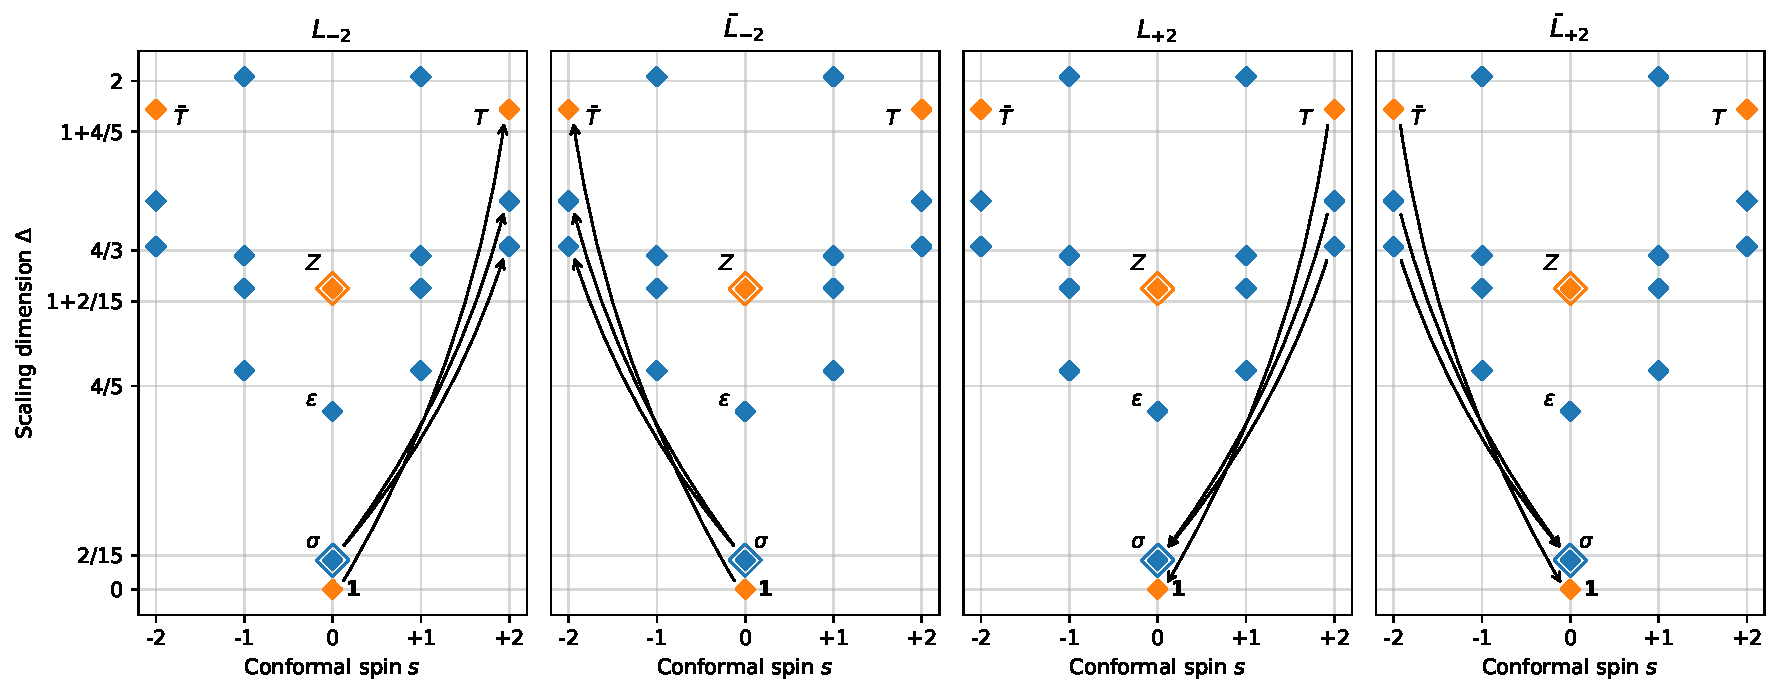
\includegraphics[width=\textwidth]{images/fibonacci/fib-virasoro-all-2.pdf}
  \caption[Virasoro 算符在 Fibonacci 模型能谱上的作用示意图]{Virasoro 算符在 Fibonacci 模型能谱上的作用示意图。图片来源:\parencite{zeng2023virasoro}。}
  \label{fig:fib-virasoro-all}
\end{figure}

\begin{sidewaystable}[ht]
  % \special{pdf: put @thispage <</Rotate 90>>}
  \centering
  \begin{tabular}{*{9}{c}}
    \toprule
      \diagbox{自旋}{标度维数}{圆柱尺寸}
                  & 4        & 8        & 12       & 16       & 20       & 24       & $\infty$     & 理论值 \\
    \midrule
      0           & 0.123499 & 0.124606 & 0.124823 & 0.124900 & 0.124936 & 0.124955 & 0.12522\,(6) & $\frac18$     \\
      0           & 1.026740 & 1.006488 & 1.002868 & 1.001610 & 1.001030 & 1.000715 & 0.9961\,(11) & 1             \\
      $\pm1$      & 1.245699 & 1.151345 & 1.136446 & 1.131388 & 1.129074 & 1.127824 & 1.107\,(5)   & $1{+}\frac18$ \\
      $\pm1,\pm2$ & 2.569513 & 2.098365 & 2.041544 & 2.022974 & 2.014590 & 2.010090 & 1.916\,(30)  & 2             \\
      0           & 2.367899 & 2.178085 & 2.148069 & 2.137876 & 2.133212 & 2.130692 & 2.089\,(11)  & $2{+}\frac18$ \\
      $\pm2$      & -        & 2.369005 & 2.223018 & 2.178379 & 2.158670 & 2.148201 & 2.043\,(19)  & $2{+}\frac18$ \\
    \bottomrule
  \end{tabular}
  \caption[Ising 模型的能谱数据]{Ising 模型的能谱数据。圆柱(转移矩阵)的尺寸 $n$ 由 4 取到 24,并且外推至无穷大。注意此处 $\Delta_\alpha$ 没有根据 $\Delta_T=2$ 的性质来进行标定。}
  \label{tab:ising-spectrum}
\end{sidewaystable}

\begin{sidewaystable}[ht]
  % \special{pdf: put @thispage <</Rotate 90>>}
  \centering
  \begin{threeparttable}
    \catcode`\"=\active
    \def"#1"{\textbf{#1}}
    \def\TPTtagStyle#1{\textit{#1}}
    \begin{tabular}{*{11}{c}}
      \toprule
        \diagbox{自旋}{标度\\[-0.5ex]维数}{圆柱\\[-0.5ex]尺寸}
                     &  9                  &  12        &  15        &  18        &  21        &  24        &  27        &  $\infty$     &  调整值       &  理论值 \\
      \midrule
        "0"          & "0.0"               & "0.0"      & "0.0"      & "0.0"      & "0.0"      & "0.0"      & "0.0"      & "0.0"         & "0.0"         & "0"                       \\
         0\tnote{a}  &  0.112899           &  0.113952  &  0.114474  &  0.114769  &  0.114950  &  0.115070  &  0.115152  &  0.11610\,(7) &  0.1513\,(32) &  $\frac{2}{15}$           \\
         0           &  0.722756           &  0.709100  &  0.703083  &  0.699890  &  0.697989  &  0.696765  &  0.695931  &  0.6856\,(9)  &  0.894\,(19)  &  $\frac45$                \\
         $\pm1$      &  0.785553           &  0.817591  &  0.841528  &  0.859630  &  0.873686  &  0.884880  &  0.893989  &  0.9557\,(27) &  1.246\,(27)  &  $1{+}\frac{2}{15}$       \\
         $\pm1$      &  1.594955           &  1.346025  &  1.242196  &  1.184631  &  1.147942  &  1.122492  &  1.103796  &  0.914\,(11)  &  1.191\,(29)  &  $1{+}\frac{2}{15}$       \\
        "0"\tnote{a} & "1.290074"          & "1.222673" & "1.196184" & "1.182805" & "1.175050" & "1.170137" & "1.166820" & "1.123\,(4)"  & "1.464\,(32)" & "$\frac{\text4}{\text3}$" \\
         $\pm1$      &  1.147427           &  1.222649  &  1.274342  &  1.312081  &  1.340887  &  1.363620  &  1.382029  &  1.510\,(4)   &  1.97\,(4)    &  $1{+}\frac45$            \\
         $\pm1$      &  3.221770           &  2.490495  &  2.169235  &  2.016147  &  1.925379  &  1.865017  &  1.821876  &  1.31\,(5)    &  1.70\,(8)    &  $1{+}\frac45$            \\
        "\textpm2"   & "2.727358"\tnote{b} & "2.139950" & "1.967143" & "1.887302" & "1.842910" & "1.815429" & "1.797149" & "1.535\,(33)" & "2.00\,(6)"   & "2"                       \\
         $\pm2$      &  1.032723\tnote{b}  &  1.178227  &  1.276463  &  1.348394  &  1.403716  &  1.447739  &  1.483672  &  1.730\,(9)   &  2.25\,(5)    &  $2{+}\frac{2}{15}$       \\
         $\pm2$      &  -\tnote{b}         &  1.430687  &  1.484488  &  1.527193  &  1.561317  &  1.589035  &  1.611935  &  1.759\,(9)   &  2.29\,(5)    &  $2{+}\frac{2}{15}$       \\
      \bottomrule
    \end{tabular}
    \begin{tablenotes}
      \item[a] 这些能级带有二重简并。
      \item[b] 对于 $n=9$ 的情况,转移矩阵不够大,因此一些高能级的后代没有出现;同时,自旋 $\pm2$ 会退化为 $\pm1$。
    \end{tablenotes}
    \caption[Fibonacci 模型的能谱数据]{Fibonacci 模型的能谱数据。真空态及其后代(标记为粗体)通过对角化带有幂等元的转移矩阵确定,见 \ref{subsec:topological-projectors} 小节。$n=\infty$ 处的数据通过对尺寸由 12 到 27 的圆柱(转移矩阵)本征值外推得到。}
    \label{tab:fib-spectrum}
  \end{threeparttable}
\end{sidewaystable}
